\documentclass[submit]{harvardml}

\course{CS181-S20}
\assignment{Assignment \#4}
\duedate{11:59pm March 27, 2020} 

\usepackage[OT1]{fontenc}
\usepackage[colorlinks,citecolor=blue,urlcolor=blue]{hyperref}
\usepackage[pdftex]{graphicx}
\usepackage{graphicx}
\usepackage{caption}
\usepackage{fullpage}
\usepackage{soul}
\usepackage{amsmath}
\usepackage{amssymb}
\usepackage{color}
\usepackage{todonotes}
\usepackage{listings}
\usepackage{common}

\usepackage[mmddyyyy,hhmmss]{datetime}

\definecolor{verbgray}{gray}{0.9}

\lstnewenvironment{csv}{
  \lstset{backgroundcolor=\color{verbgray},
  frame=single,
  framerule=0pt,
  basicstyle=\ttfamily,
  columns=fullflexible}}{}
 
\begin{document}

\begin{center}
{\Large Homework 4: SVM, Clustering, and Ethics}\\
\end{center}

\subsection*{Introduction}

This homework assignment will have you work with SVMs, 
clustering, and engage with the ethics lecture.  

Please submit the \textbf{writeup PDF to the Gradescope assignment `HW4'}. Remember to assign pages for each question.

Please submit your \textbf{\LaTeX\ file and code files to the Gradescope assignment `HW4 - Supplemental'}. 

You can use a \textbf{maximum of 2 late days} on this assignment.  Late days will be counted based on the latest of your submissions. 

\newpage

%%%%%%%%%%%%%%%%%%%%%%%%%%%%%%%%%%%%%%%%%%%%%
% Problem 1
%%%%%%%%%%%%%%%%%%%%%%%%%%%%%%%%%%%%%%%%%%%%%
\begin{problem}[Fitting an SVM by hand, 10pts]

  For this problem you will solve an SVM by hand, relying on principled rules and SVM properties. 
  For making plots, however, you are allowed to use a computer or other graphical tools.

Consider a dataset with the following 7 data points each with $x \in \reals$ and $y \in \{ -1, +1 \}$ : \[\{(x_i, y_i)\}_{i = 1}^7 =\{(-3 , +1) , (-2 , +1 ) , (-1,  -1 ), (0, +1), ( 1 , -1 ), ( 2 , +1 ) , (3 , +1 )\}\] Consider
mapping these points to $2$ dimensions using the feature vector $\bphi(x) =  (x, -\frac{8}{3}x^2 + \frac{2}{3}x^4 )$. The hard margin classifier training problem is:
%
\begin{align*}
  &\min_{\mathbf{w}, w_0} \|\mathbf{w}\|_2^2 \label{eq:dcp} \\
  \quad \text{s.t.} \quad & y_i(\mathbf{w}^\top \bphi(x_i) + w_0) \geq 1,~\forall i \in \{1,\ldots, n\}\notag
\end{align*}

Make sure to follow the logical structure of
the questions below when composing your answers, and to justify each step.

\begin{enumerate}
\item Plot the transformed training data in $\reals^2$ and draw the optimal decision boundary
of the max margin classifier. You can determine this by inspection (i.e. by hand, without actually doing any calculations).

\item  What is the value of the margin achieved by the optimal
decision boundary found in Part 1? 

\item Identify a unit vector that is orthogonal to the decision boundary.

\item Considering the discriminant $h(\bphi(x);\boldw,w_0)=\boldw^\top\bphi(x) +w_0$, 
give an expression for {\em all possible} $(\boldw,w_0)$ that define
the decision boundary. Justify your answer.

  \item Consider now the training problem for this dataset. Using your answers so far,
    what particular solution to $\boldw$ will be optimal for the
    optimization problem?

  \item What is the corresponding optimal value of $w_0$ for the $\boldw$ found in Part 5 (use your result from Part 4 as guidance)? Substitute in these optimal values and write out the discriminant function
    $h(\bphi(x);\boldw,w_0)$ in terms of the variable $x$ .


\item What are the support vectors of the classifier?  Confirm that
  the solution in Part 6 makes the constraints above binding for these
  support vectors.

\end{enumerate}

\end{problem}

\newpage

\subsection*{Solution}

\begin{enumerate}
    \item This is what the transformed data looks like one plotted. Upon inspection we have plotted the optimal decision boundary at $\phi_{2}(x)= -1$. \newline
    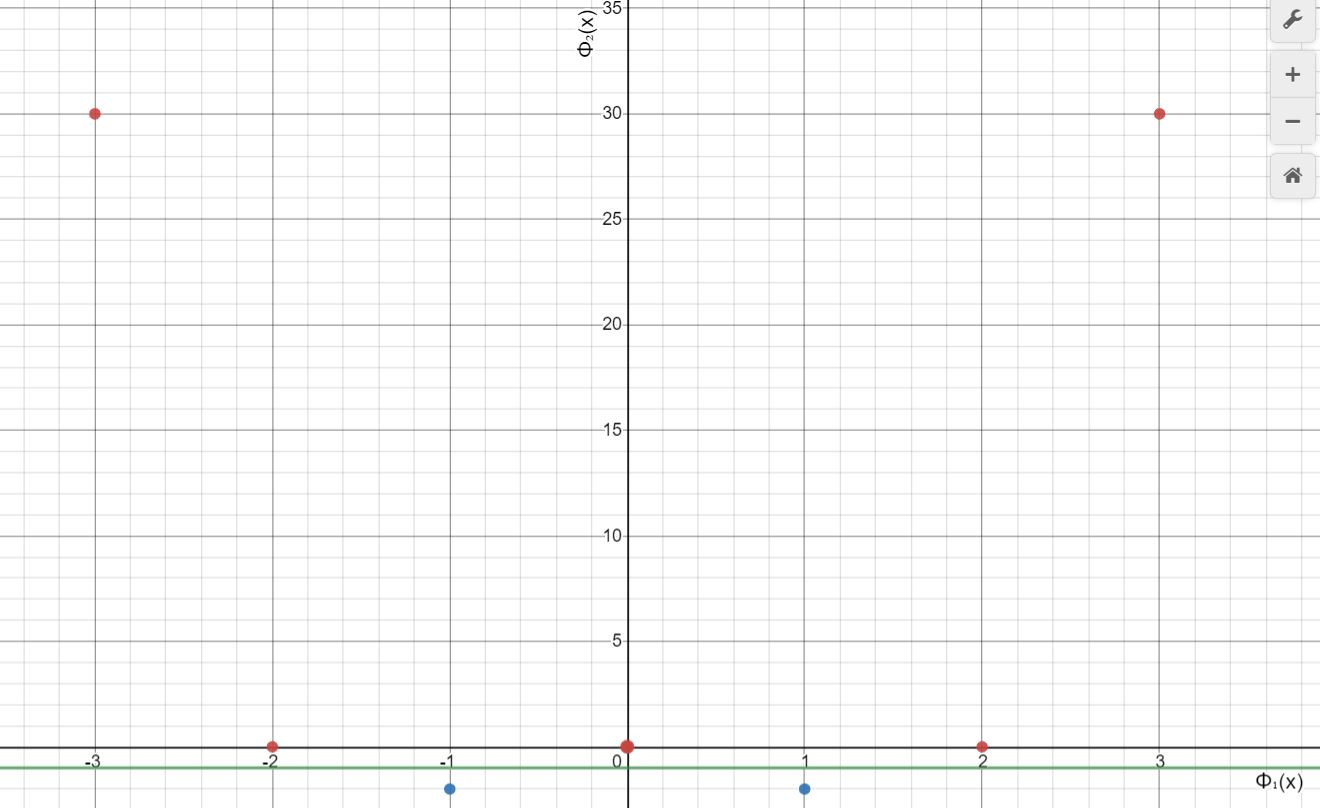
\includegraphics[scale=.50]{hw4/Pics/graph1_hw4.JPG}
    
    \item The margin achieved by the optimal decision boundary is 1.
    
    \item $\begin{bmatrix}
           0 \\
           1 \\
         \end{bmatrix}$
         is orthogonal to the decision boundary. 
         
    \item
        $\boldw = \begin{bmatrix}
           0 \\
           1 \\
         \end{bmatrix}$
         \begin{equation*}
             h(\phi(x); \boldw, w_0) = [0,1]\phi(x) + w_0 = 0
         \end{equation*}
         \begin{equation*}
             h(\phi(x); \boldw, w_0) = [0,1][\phi_{1}(x), \phi_{2}(x)] + w_0
         \end{equation*}
         \begin{center}
             We know that $\phi_{2}(x) = -1$  is the decision boundary. We can now substitute.
         \end{center}
         \begin{equation*}
             h(\phi(x); \boldw, w_0) = [0,1][\phi_{1}(x), -1] + w_0
         \end{equation*}
         \begin{center}
             From here we can now simplify.
         \end{center}
         \begin{equation*}
             h(\phi(x); \boldw, w_0) = -1 + w_0 = 0
         \end{equation*}
         \begin{equation*}
             w_0 = 1
         \end{equation*}
         From here we get that $\boldw = \begin{bmatrix}
           0 \\
           1 \\
         \end{bmatrix}$, $w_0 = 1$ is a valid ($\boldw, w_0$). The discriminant equation is not affected by scaling since it equals 0. So for some $\boldw_{c}$ and $w_{0,c}$ we have $\boldw_{c} = c\boldw$ and $w_{0,c} = cw_0$ and these are valid combinations of $\boldw$ and $w_0$. So from this we can conclude that any combination of this form is valid. Therefore, the general form can be described by ($\boldw =
         \begin{bmatrix}
           0 \\
           c \\
         \end{bmatrix}$, $w_0 = c$).
         
    \item
        We can solve this by looking at $y_i(\mathbf{w}^\top \bphi(x_i) + w_0) \geq 1$ which is the constratint on the minimization of the norm of $\boldw$. This should hold for all support vectors, so we can chose one of the point closest to our boundary. So we can choose $(-1, -1)$ and transform with $\phi(x)$ which gives $(-1, -2)$ and then solve using the result from part 4.
        
        \begin{equation*}
            y_i(\mathbf{w}^\top \bphi(x_i) + w_0) \geq 1
        \end{equation*}
        \begin{equation*}
            -1([0, c][-1, -2] + c) = 1
        \end{equation*}
        \begin{equation*}
            -2c + c = -1
        \end{equation*}
        \begin{equation*}
            c = 1
        \end{equation*}
        
        And so we get that $\boldw = \begin{bmatrix}
        0 \\
        1 \\
        \end{bmatrix}$ is the optimal solution for the optimization problem.
        
        \item Our solution for part 5 already solves for c so we get our optimal value of $w_0 = 1$, this agrees with part 4.
        
        So our discriminant function now looks like $h(\bphi(x);\boldw,w_0) = [0, 1]\phi(x) + 1$
        
        \item We can easily identify the support vectors from the graph. The five are (-2,0), (-1,-2), (0,0), (1,-2), (2, 0), these are given transformed by $\phi(x)$.
        
        Now we use $y_i(\mathbf{w}^\top \bphi(x_i) + w_0) = 1$ to confirm the constraints are binding.
        \begin{equation*}
            (-2,0) : 1([0,1][-2,0] + 1) = 1 \longrightarrow True
        \end{equation*}
        \begin{equation*}
            (-1,-2) : -1([0,1][-1,-2] + 1) = 1 \longrightarrow True
        \end{equation*}
        \begin{equation*}
            (0,0) : 1([0,1][0,0] + 1) = 1 \longrightarrow True
        \end{equation*}
        \begin{equation*}
            (1,-2) : -1([0,1][1,-2] + 1) = 1 \longrightarrow True
        \end{equation*}
        \begin{equation*}
            (2, 0) : 1([0,1][2,0] + 1) = 1 \longrightarrow True
        \end{equation*}
\end{enumerate}
%%%%%%%%%%%%%%%%%%%%%%%%%%%%%%%%%%%%%%%%%%%%%
% Problem 2
%%%%%%%%%%%%%%%%%%%%%%%%%%%%%%%%%%%%%%%%%%%%%
\begin{problem}[K-Means and HAC, 20pts]


For this problem you will implement K-Means clustering and HAC from
scratch. Using \texttt{numpy} is fine, but don't use a third-party
machine learning implementation like \texttt{scikit-learn}. You will
then apply this approach to the clustering of image data.

We've provided you with a subset of the MNIST dataset, a collection of
handwritten digits used as a benchmark for image recognition (you can
learn more about the data set at
\url{http://yann.lecun.com/exdb/mnist/}). The MNIST task is widely
used in supervised learning, and modern algorithms do very well.

Here you will apply unsupervised learning to MNIST. You have been given
representations of MNIST images, each of which is a $784\times1$
greyscale handwritten digit from 0-9. Your job is to implement K-means
clustering and HAC on MNIST, and to test whether these relatively
simple algorithms can cluster similar-looking images together.

The code given in \texttt{T4\_P2.py} loads the images into your environment into two arrays -- \texttt{large\_dataset} is a 5000x784 array that should be used for K-means, while \texttt{small\_dataset} is a 300x784 array that will be used for HAC clustering. In your code, you should use the $\ell_2$ norm (i.e. Euclidean distance) as your distance metric.

\textbf{Important:} Remember to include all of your plots in your PDF submission!

\begin{enumerate}

\item Starting at a random initialization and $K = 10$, plot
  the K-means objective function (the residual sum of squares) as a function of iterations and verify
  that it never increases.

\item Run the K-means algorithm for 5 different restarts for different
  values of $K$, setting $K = 5, 10, 20$. Plot the final K-means objective value as a function
  of $K$ with error bars over the $5$ random restarts. To clarify, your
  x-axis will be $K$, your y-axis will be the average objective function value
  after your algorithm converges, and each data point will have an
  error bar -- to calculate these error bars you must run your K-means
  algorithm $5$ times for each $K$ (giving you multiple final objective values
  for each $K$) then use these values to calculate a standard deviation for
  each $K$ before plotting error bars around each data point. How
  does the final value of the objective function and the standard deviation of the final
  value of the objective function change with $K$? (Note: Our code takes ~10 minutes to run for this Part)
  
\item For $K=10$ and for 5 random restarts, show the mean
  image (aka the centroid) for each cluster.
  To render an image, use the pyplot
  \texttt{imshow} function. There should be 50 total images. Include all of these images
  as part of a single plot (e.g. don't have 50 pages in your write-up with a
  separate image on each page).

\item Repeat Part 3, but first standardize the data. That is, center
  the data before running K-means on it, such that each pixel has mean 0 and variance 1 (except
  for any pixels that have zero variance, for these you can simply
  divide by 1). For $K=10$ and 5 random restarts, show the mean image
  (aka the centroid) for each cluster. There should be 50 total
  images. Again, include all of these images as part of a single plot.
  Compare these images to those from Part 3.

\item Implement HAC for min, max, and centroid-based linkages. Fit these models to the \texttt{small\_dataset} images. 
  For each of these 3 linkage criteria, find the mean image for each cluster when using $10$ clusters, and display these images on a plot. There should be 30 total images.
  How do these mean images compare to those found with K-means? \textbf{Important Note:} For this part only, you may use the \texttt{scipy} package's \texttt{cdist} function to calculate the Euclidean distances between every pair of points in two arrays. DO NOT use \texttt{scipy} for anything else. 

\item For each of the 3 HAC linkages (max/min/centroid), make a plot of
  ``Distance between most recently merged clusters" (y-axis) v. ``Total number of merges completed" (x-axis).
  Does this plot suggest that there are any  natural cut points? 

\item Re-fit a K-means with $K = 10$ model and HAC min/max/centroid models using $10$ clusters on the \texttt{small\_dataset} images. Use the \texttt{seaborn} module's \texttt{heatmap} function to plot a confusion matrix of clusters v. actual digits, i.e. the cell at the $i$th row, $j$th column of your confusion matrix should be the number of times that an image with the true label of $j$ appears in cluster $i$. How well do the different approaches match the digits? Is this matching a reasonable evaluation metric for the clustering?  Explain why or why not.  
  
\end{enumerate}

\end{problem}

\newpage

\subsection*{Solution}
\begin{enumerate}
    \item Upon inspection we can see that it does not increase.\newline
    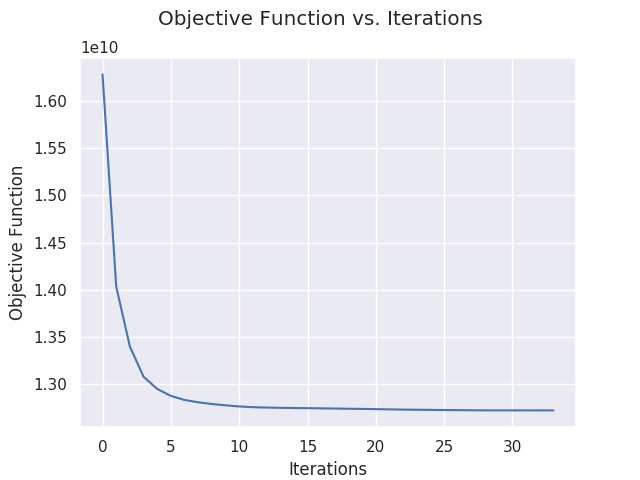
\includegraphics[scale=.70]{hw4/Pics/Part1.png}
    
    \item As $K$ increases the final value of the objective function and the standard deviation decrease. \newline
    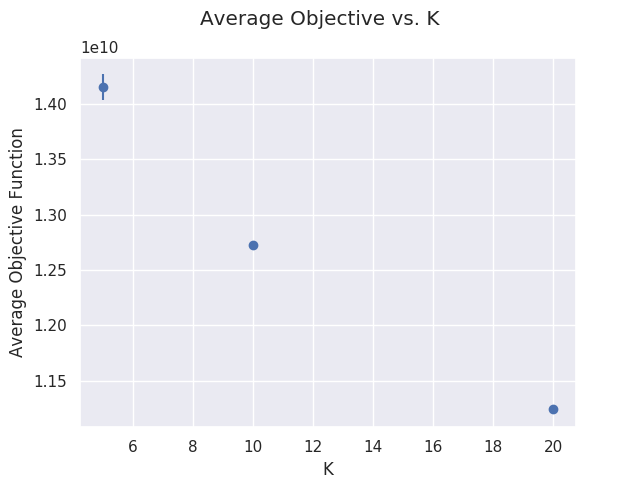
\includegraphics[scale=.70]{hw4/Pics/Part2.png}
    \newpage
    \item\hspace{2 cm}Restart 1\hspace{1 cm}Restart 2\hspace{1 cm}Restart 3\hspace{1 cm}Restart 4\hspace{1 cm}Restart 5 \newline
    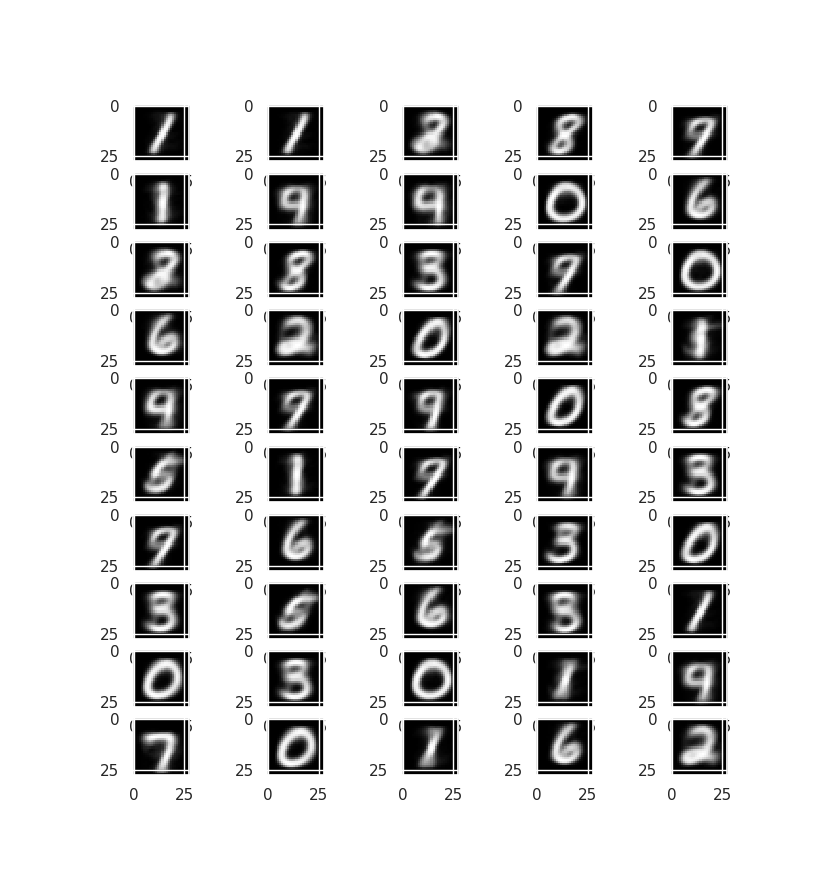
\includegraphics[scale=.70]{hw4/Pics/Part3.png}\newline
    \newpage
    \item\hspace{2.4 cm}Restart 1\hspace{1 cm}Restart 2\hspace{1 cm}Restart 3\hspace{1 cm}Restart 4\hspace{1 cm}Restart 5 \newline
    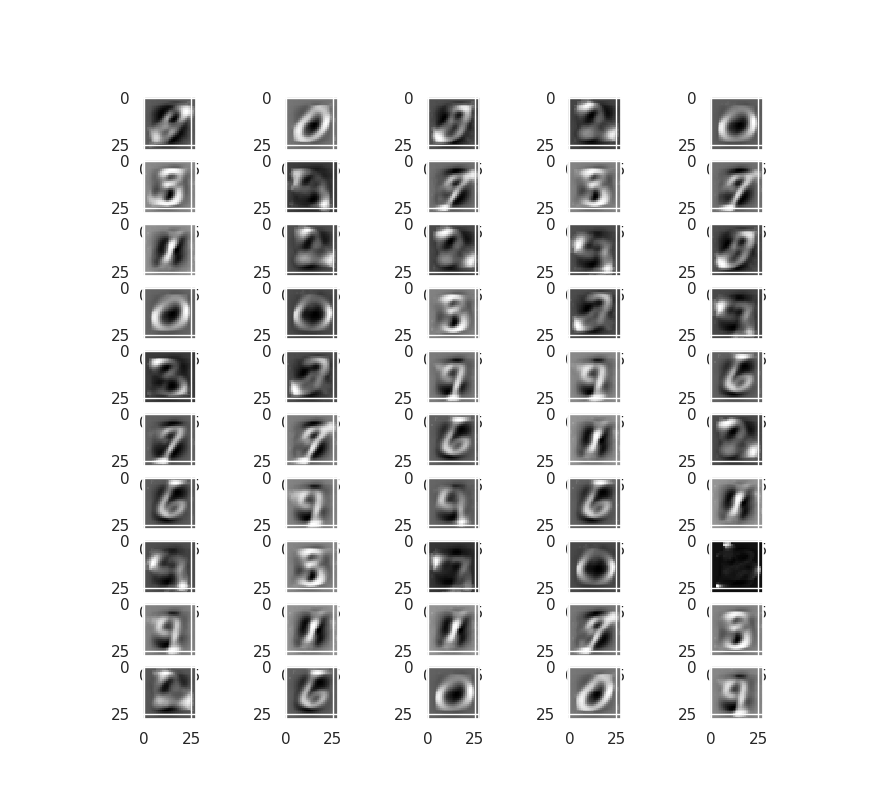
\includegraphics[scale=.70]{hw4/Pics/Part4.png}\newline
    The images in part 3 (non-standardized) very clearly appear to be numbers. While the images in part 4 (standardized) look somewhat like numbers but then appear to have a blur or indistinctness to them. After some research this is caused by the way negative numbers are treated when graphing. When we subtracted the mean to standardize we got some negative numbers, and when those were graphed they were treated as zeros and everything else was scaled accordingly which is why we get this blurry semblance of a number.
    \newpage
    \item \hspace{3.5cm}min\hspace{3.7 cm}max\hspace{3.5 cm}centroid\newline
    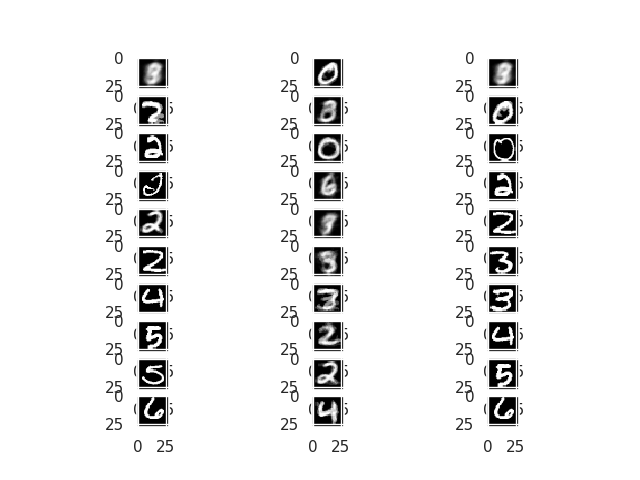
\includegraphics[scale=1.0]{hw4/Pics/Part5.png}\newline
    For all the images created by the different HAC linkages when there is a number it is much crisper and more easily identifiable when compared to K-means. This is less the case in much of the max linkage (but it does still does occur to some extent). It  seems like the HAC method is able to create much more accurate clusters (when using the right linkage) than K-means.
    \newpage
    \item \hspace{1 cm} \newline
    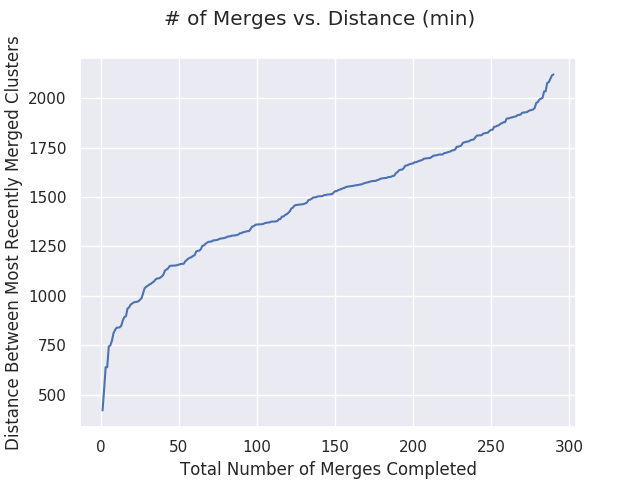
\includegraphics[scale=.70]{hw4/Pics/Part6-1.png}\newline
    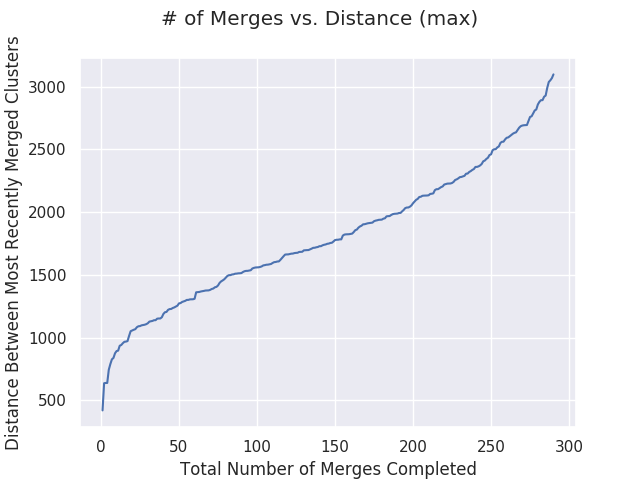
\includegraphics[scale=.70]{hw4/Pics/Part6-2.png}\newline
    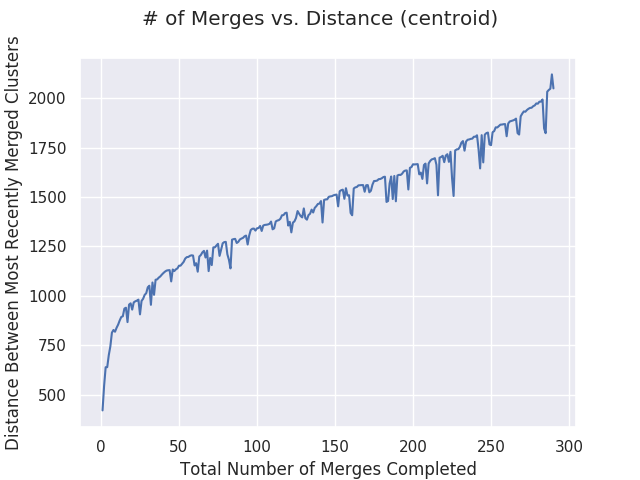
\includegraphics[scale=.70]{hw4/Pics/Part6-3.png}\newline
    For all three of the graphs the natural cut points seem to be around 280 or so merges. 
    \item \hspace{1 cm} \newline
    \begin{center}
    \hspace{1cm}Heatmap for K-means\newline
    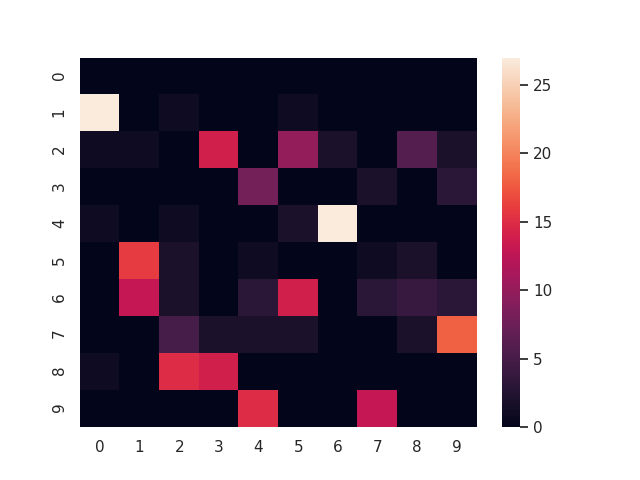
\includegraphics[scale=.70]{hw4/Pics/Part7_K.png}\newline
    Heatmap for HAC min linkage\newline
    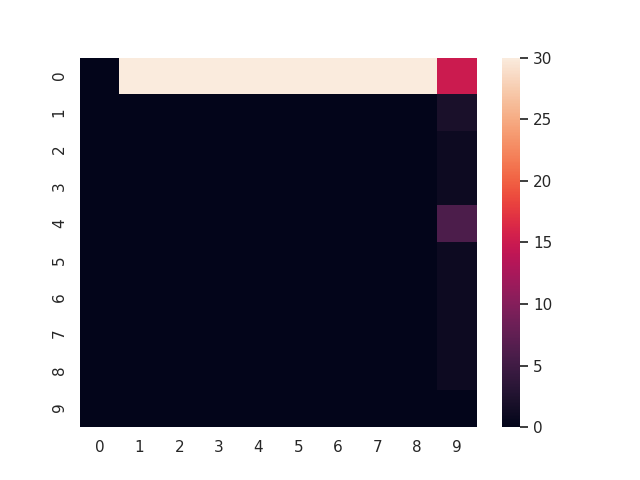
\includegraphics[scale=.70]{hw4/Pics/Part7_min.png}\newline
    Heatmap for HAC max linkage\newline
    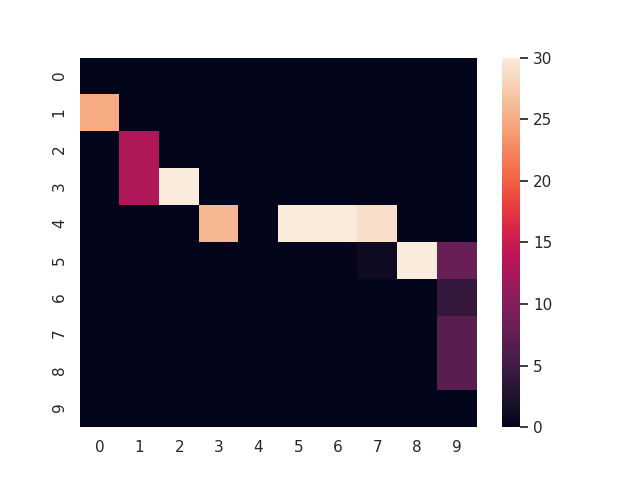
\includegraphics[scale=.70]{hw4/Pics/Part7_max.png}\newline
    \newpage
    Heatmap for HAC centroid linkage\newline
    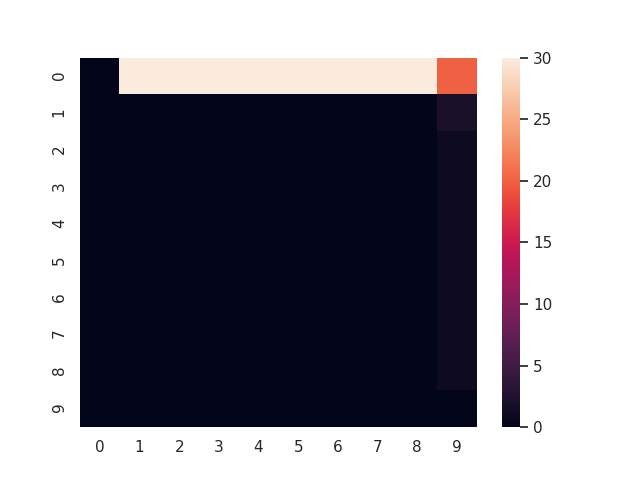
\includegraphics[scale=.70]{hw4/Pics/Part7_cent.png}\newline
    \end{center}
    According to this the K-means approach is a bit all over the place in terms of correctly matching. And the HAC approaches all have specific areas of issue at 0 for min and max linkages and at 4 for the centroid linkage. So I would say that the HAC min and max match the best, followed by the K-means, and then in last is the HAC centroid.
    
    I do not believe this is a reasonable evaluation metric for the clustering since due to manipulation of the data and the way means and other variables are initialized the class that is labeled 4 in our program might not correspond to the data that has a label of 4 which leads to confusion when you compare the clustering approach. This will likely lead to an incorrect assessment of which method works best and delivers the best results.
\end{enumerate}

\newpage
%%%%%%%%%%%%%%%%%%%%%%%%%%%%%%%%%%%%%%%%%%%%%
% Problem 3
%%%%%%%%%%%%%%%%%%%%%%%%%%%%%%%%%%%%%%%%%%%%%
\begin{problem}[Ethics Assignment, 15pts]
Imagine that you are a product manager in a technology company and the board of directors requests a detailed report of the potential social impact of the product you're building. You are currently working on an algorithm designed to allocate economic resources for various health providers. You are instructed to address various kinds of possible impacts, giving special attention to the algorithm’s potential to wrongfully discriminate against vulnerable populations. 

Having followed the coding process closely, you can confidently assume that there is no discriminatory intent animating the design.  In fact, the product’s design is based on the notion that resources should be distributed to health centers in a manner that is proportional to the needs of the populations they attend to. However, you worry that there may still be wrongful discrimination due to disparate negative impact on members of low-income populations, migrants, and racial minorities. 

What further questions must you address in order to confidently determine whether the algorithm wrongfully discriminates against members of these groups? Write two questions and, for each, write a short paragraph explaining how addressing this question can help you assess the algorithm’s potential for wrongful discrimination.


We expect clear, concise, and thoughtful engagement with this question, which includes providing your reasoning for your answers.  In your response, depth is more important than breadth. We do \emph{not} expect you to do any outside research, though we encourage you to connect to lecture materials where relevant.

\end{problem}
\newpage
\subsection*{Solution}
     
    These vulnerable population are typically less likely to go to health centers and as such the actual need in a given area may under-reported. Does the algorithm factor this into account using other metrics?
     \vspace{.5cm}
     
    This question lets us know whether or not the algorithm is taking into account a wide range of data that can account for or mitigate inconsistencies in reporting practices (that can come from malice or disorganization). It also allows us to see if population counts are be taken into account when resources are allocated. In taking these metrics into account so we can combat under-reporting we attempt to minimize the potential for discrimination. As these are key points to look into because if the algorithm failed to take this into account then in reality it is not accomplishing its main goal. Once we address this question we know if we need to add more data to the model or tweak how the data is manipulated/handled by the model and in doing so the potential for wrongful discrimination due to this facet would be less likely.
    \vspace{.5cm}
    \newline
    Upon testing does the algorithm allocate more resources to wealthier or more well off communities in comparison to those communities with more vulnerable populations?
    \vspace{.5cm}
    
    This is a question to be addressed in the earlier testing phases. This question really lets us known whether or not their are inherent biases in the data we are giving the algorithm, that the algorithm by its nature is reinforcing. If the algorithm did end up not allocating resources to areas that are well understood to need the resources or if it allocated resources to areas that are known to not need it then we would know in the early stages that there is a major issue with the data (whether it be bias, lack of variety of data, or something else altogether). From there the algorithm can be readjusted and retested until it performs more correctly. By doing this we can assure ourselves that the a design we are implementing benefits vulnerable groups rather than increase the inequality they experience. In addition, by doing this in the early stages the hope is we mitigate any unknown discrimination from existing and potentially continuing to propagate into other models.
    
\newpage
%%%%%%%%%%%%%%%%%%%%%%%%%%%%%%%%%%%%%%%%%%%%%
% Name and Calibration
%%%%%%%%%%%%%%%%%%%%%%%%%%%%%%%%%%%%%%%%%%%%%
\subsection*{Name}
Jason Sibrian

\subsection*{Collaborators and Resources}
Whom did you work with, and did you use any resources beyond cs181-textbook and your notes?
\newline
N/A

\subsection*{Calibration}
Approximately how long did this homework take you to complete (in hours)? 
\newline
25

\end{document}
